\documentclass[runningheads]{llncs}

\usepackage[T1]{fontenc}
\usepackage{graphicx}
\usepackage{url}
\usepackage{hyperref}
\usepackage{booktabs}
\usepackage{multirow}

\begin{document}

\title{Classification of Selected Philippine Bird Species Using Acoustic Features and Classical Machine Learning}
\titlerunning{Philippine Bird Species Classification}

\author{Emmanuel Albeza \and Yvonne Lin \and Christalie Pategara}
\authorrunning{E. Albeza et al.}

\institute{
University of the Philippines Visayas\\
\email{eaalbeza@up.edu.ph, yalin@up.edu.ph, chpategara@up.edu.ph}
}

\maketitle

\begin{abstract}
This study developed a classical machine learning approach for classifying selected Philippine bird species from audio recordings. Recordings were collected from the Xeno-canto bird sound repository and processed into standardized audio clips. Acoustic features, including Mel-frequency cepstral coefficients, spectral descriptors, and temporal features, were extracted and used to train traditional machine learning classifiers. The evaluated models included Logistic Regression, Support Vector Machine, Random Forest, Extra Trees, Gradient Boosting, K-Nearest Neighbors, and XGBoost. Results showed that tree-based ensemble models performed competitively in cross-validation. The final model achieved an accuracy of 0.7465, approximately 75\%, and a macro F1-score of 0.74 on a held-out test set of 71 recordings. These results suggest that handcrafted acoustic features combined with classical machine learning can provide a feasible baseline for Philippine bird species classification, although performance remains limited by dataset size, recording noise, and species-level acoustic similarity.

\keywords{bird sound classification \and acoustic features \and machine learning \and Philippine birds \and passive acoustic monitoring}
\end{abstract}

\section{Introduction}

Bird vocalizations are an important source of information for biodiversity monitoring because many bird species can be detected through their calls and songs even when they are difficult to observe visually. Passive acoustic monitoring provides a non-invasive way to record animal sounds across different locations and time periods, allowing researchers to collect ecological information with less dependence on continuous human observation \cite{szymanski2021,biffi2024,mosikidi2023}. However, the manual identification of species from large volumes of audio recordings can be time-consuming and requires domain expertise.

Automated bird sound classification can help address this challenge by using computational models to identify species from recorded vocalizations. Such systems may support biodiversity monitoring, ecological research, and assisted species identification. In the Philippine context, bird sound classification is especially relevant because the country has high avian diversity and many species of ecological interest. Developing computational tools for selected Philippine bird species can therefore contribute to broader efforts in biodiversity assessment and conservation-oriented monitoring.

This study focused on the classification of selected Philippine bird species using handcrafted acoustic features and classical machine learning models. Audio recordings were obtained from the Xeno-canto repository, a public archive of wildlife sound recordings and associated metadata \cite{xenocanto}. The study extracted Mel-frequency cepstral coefficients (MFCCs), spectral features, and temporal features from the recordings. These features were then used to train and compare several traditional machine learning classifiers.

The main objective of this study was to evaluate whether classical machine learning models using handcrafted audio features can provide a feasible baseline for selected Philippine bird species classification. Specifically, the study aimed to: (1) curate a dataset of selected Philippine bird species from Xeno-canto, (2) extract acoustic features from the audio recordings, (3) compare multiple classical machine learning classifiers, and (4) evaluate the final model using accuracy, precision, recall, macro F1-score, and a confusion matrix.

\section{Related Work}

Bird sound classification has been studied using both traditional machine learning and more recent deep learning approaches. Earlier works commonly used handcrafted acoustic features together with classifiers such as Support Vector Machines. Fagerlund \cite{fagerlund2007} showed that bird species recognition can be performed using low-level audio parameters and mel-cepstral features. These types of features are useful because they summarize the spectral and temporal characteristics of bird vocalizations in a numerical form that can be used by machine learning models.

Mel-frequency cepstral coefficients have been widely used in audio classification tasks because they represent the short-term spectral properties of sound in a compact feature vector. MFCCs are commonly used in speech and bioacoustic recognition tasks, including bird sound classification \cite{librosa_mfcc,fagerlund2007}. In bird classification, MFCCs can capture differences in frequency structure, timbre, and vocal patterns across species.

Traditional machine learning models remain useful for small to medium-sized datasets because they are generally easier to train and interpret than deep neural networks. Models such as Logistic Regression, Support Vector Machines, Random Forest, Extra Trees, Gradient Boosting, K-Nearest Neighbors, and XGBoost can be trained on handcrafted audio features. Recent studies have also compared MFCC-based features with classifiers such as SVM and Random Forest for bird sound recognition tasks \cite{han2023}. These studies show that traditional models can still provide meaningful baselines, especially when the dataset size is limited.

This study builds on previous work by applying classical machine learning models to selected Philippine bird species. Instead of using deep learning, the project focuses on a reproducible pipeline using curated audio recordings, handcrafted acoustic features, cross-validation, hyperparameter tuning, and held-out test evaluation.

\section{Methodology}

The study followed a structured machine learning workflow consisting of dataset collection, pre-processing, feature extraction, model training, hyperparameter tuning, and final evaluation.

\subsection{Dataset Collection}

Audio recordings were collected from Xeno-canto, a public online repository of wildlife sound recordings \cite{xenocanto}. The dataset was limited to selected bird species with recordings associated with the Philippines. The species were selected based on recording availability, usability of audio quality, and class balance.

The final classification task consisted of five Philippine bird species:

\begin{itemize}
    \item \textit{Hypsipetes philippinus}
    \item \textit{Phapitreron leucotis}
    \item \textit{Dicrurus balicassius}
    \item \textit{Ninox philippensis}
    \item \textit{Brachypteryx montana}
\end{itemize}

The dataset was prepared as a five-class classification problem. Metadata cleaning and filtering were performed to remove unusable or unidentified recordings. The curated dataset was then used for pre-processing and feature extraction.

\subsection{Pre-processing}

The raw audio recordings were standardized before feature extraction to reduce differences in file format, sampling rate, channel configuration, duration, and amplitude. Each recording was converted to mono-channel WAV format and resampled to 22{,}050 Hz. Silence trimming was applied to remove low-energy leading and trailing portions of the signal, and amplitude normalization was performed to reduce volume variation across recordings. Each clip was then adjusted to a fixed duration of 10 seconds by trimming longer recordings and padding shorter recordings when necessary.

This pre-processing step was necessary because the Xeno-canto recordings were collected by different contributors using different recording devices and under varying environmental conditions. Standardizing the audio ensured that the extracted acoustic features were computed under consistent input conditions.

\subsection{Feature Extraction}

Acoustic features were extracted from each pre-processed 10-second audio clip using \texttt{librosa}. For each recording, 20 Mel-frequency cepstral coefficients (MFCCs) were computed, together with their first-order delta and second-order delta features. Additional spectral features were extracted, including spectral centroid, spectral bandwidth, spectral rolloff, and spectral contrast. Temporal and energy-based features, including zero-crossing rate, root mean square (RMS) energy, and duration, were also computed.

Because these features vary over time, each feature sequence was summarized using four statistical descriptors: mean, standard deviation, minimum, and maximum. The resulting values were stored in a labeled feature table, where each row represented one audio recording and each column represented one numerical feature. The species name was used as the target label for model training.

\subsection{Model Training and Evaluation}

Seven classical machine learning classifiers were evaluated: Logistic Regression, Support Vector Machine with radial basis function kernel (SVM-RBF), Random Forest, Extra Trees, Gradient Boosting, K-Nearest Neighbors (KNN), and XGBoost. The feature table was split into training and held-out test sets using stratified sampling to preserve the class distribution. Model comparison was performed using stratified cross-validation on the training set.

Performance was measured using accuracy, macro precision, macro recall, macro F1-score, and confusion matrices. Macro F1-score was used as the primary selection metric because the dataset was slightly imbalanced and all bird species were considered equally important \cite{sklearn_f1}. Hyperparameter tuning was then applied to selected high-performing models, specifically XGBoost, Extra Trees, Random Forest, and SVM-RBF. The final model was selected based on cross-validation performance and evaluated on the held-out test set.

\section{Results and Discussion}

\subsection{Dataset Distribution}

The final dataset contained 354 recordings from five Philippine bird species. As shown in Figure~\ref{fig:species-distribution}, the class distribution was moderately imbalanced, with \textit{Hypsipetes philippinus} having the most recordings and \textit{Brachypteryx montana} having the fewest. This imbalance supports the use of macro-averaged metrics in addition to accuracy.

\begin{figure}
\centering
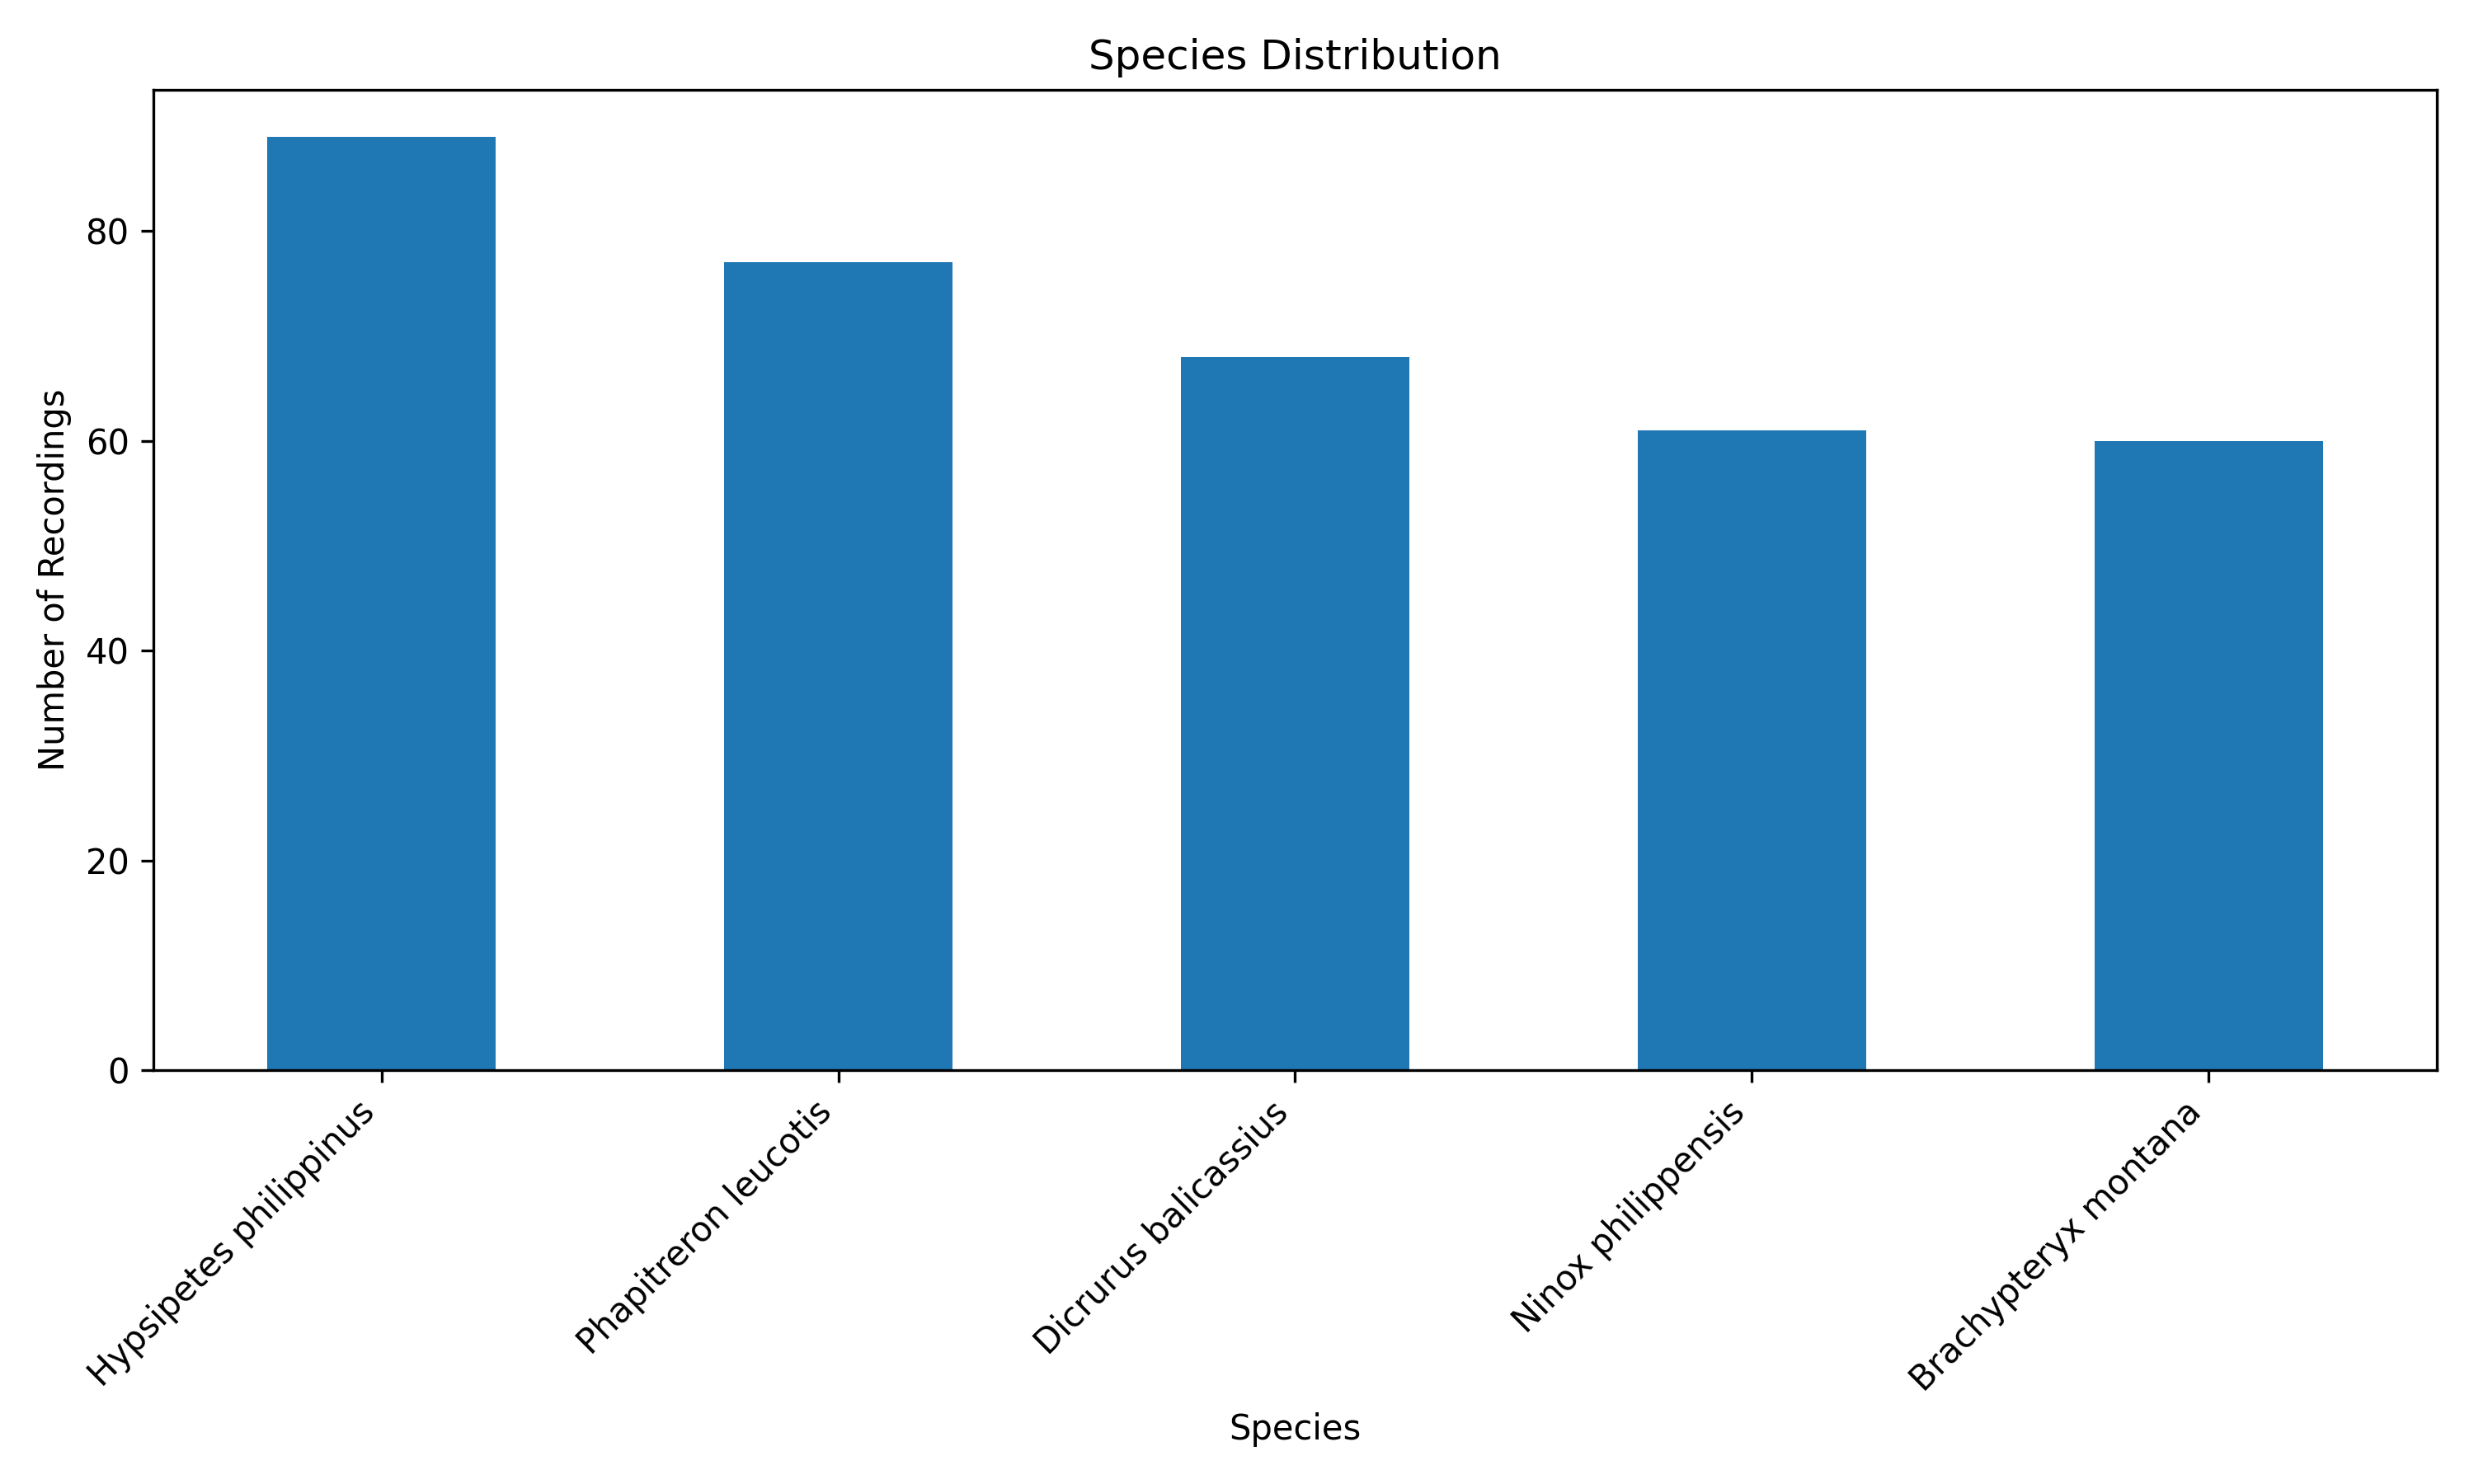
\includegraphics[width=0.80\textwidth]{figures/species_distribution.png}
\caption{Distribution of recordings across the selected Philippine bird species.}
\label{fig:species-distribution}
\end{figure}

\subsection{Cross-Validation Results}

Table~\ref{tab:cv-results} presents the stratified cross-validation results of the baseline models. Random Forest achieved the highest mean accuracy at 0.7539, while Extra Trees obtained the highest mean macro F1-score at 0.7475. Logistic Regression and XGBoost were also competitive, with macro F1-scores of 0.7471 and 0.7436, respectively. KNN produced the lowest performance, suggesting that distance-based classification was less effective for the extracted feature space.

\begin{table}
\centering
\caption{Cross-validation results of baseline models.}
\label{tab:cv-results}
\begin{tabular}{lcc}
\toprule
Model & Mean Accuracy & Mean Macro F1-score \\
\midrule
Extra Trees & 0.7504 & 0.7475 \\
Random Forest & 0.7539 & 0.7475 \\
Logistic Regression & 0.7434 & 0.7471 \\
XGBoost & 0.7434 & 0.7436 \\
SVM-RBF & 0.7329 & 0.7382 \\
Gradient Boosting & 0.7081 & 0.7073 \\
KNN & 0.6306 & 0.6345 \\
\bottomrule
\end{tabular}
\end{table}

Figure~\ref{fig:model-comparison} shows the model comparison based on macro F1-score. The close performance of Extra Trees, Random Forest, Logistic Regression, and XGBoost indicates that the extracted MFCC, spectral, and temporal features provided useful class-discriminative information. However, the relatively small gap among the top models also suggests that performance was constrained by dataset size and recording variability.

\begin{figure}
\centering

\includegraphics[width=0.90\textwidth]{figures/model_comparison.png}
\caption{Cross-validation comparison of the evaluated machine learning models.}
\label{fig:model-comparison}
\end{figure}

\subsection{Hyperparameter Tuning Results}

Table~\ref{tab:tuning-results} summarizes the best macro F1-scores obtained after hyperparameter tuning. XGBoost achieved the highest tuned cross-validation macro F1-score of 0.7714 using a learning rate of 0.1, maximum depth of 4, 100 estimators, subsample value of 0.8, and colsample\_bytree value of 0.9. Extra Trees followed with a macro F1-score of 0.7622.

\begin{table}
\centering
\caption{Hyperparameter tuning results.}
\label{tab:tuning-results}
\begin{tabular}{lc}
\toprule
Model & Best CV Macro F1-score \\
\midrule
XGBoost tuned & 0.7714 \\
Extra Trees tuned & 0.7622 \\
Random Forest tuned & 0.7537 \\
SVM-RBF tuned & 0.7503 \\
\bottomrule
\end{tabular}
\end{table}

Although tuning improved the best cross-validation score, the held-out test results remained moderate. This suggests that model performance was limited not only by hyperparameter choice, but also by the size and variability of the available recordings.

\subsection{Final Held-Out Test Results}

The final held-out test set contained 71 recordings. The final model correctly classified 53 recordings and misclassified 18, producing an accuracy of 0.7465 and a macro F1-score of 0.74. Table~\ref{tab:classification-report} presents the per-class results.

\begin{table}
\centering
\caption{Final held-out test classification report.}
\label{tab:classification-report}
\begin{tabular}{lcccc}
\toprule
Species & Precision & Recall & F1-score & Support \\
\midrule
\textit{Brachypteryx montana} & 1.00 & 0.42 & 0.59 & 12 \\
\textit{Dicrurus balicassius} & 0.67 & 0.43 & 0.52 & 14 \\
\textit{Hypsipetes philippinus} & 0.52 & 0.89 & 0.65 & 18 \\
\textit{Ninox philippensis} & 1.00 & 0.92 & 0.96 & 12 \\
\textit{Phapitreron leucotis} & 1.00 & 1.00 & 1.00 & 15 \\
\midrule
Accuracy & \multicolumn{3}{c}{0.75} & 71 \\
Macro average & 0.84 & 0.73 & 0.74 & 71 \\
Weighted average & 0.81 & 0.75 & 0.74 & 71 \\
\bottomrule
\end{tabular}
\end{table}

The model performed best on \textit{Phapitreron leucotis} and \textit{Ninox philippensis}, which achieved F1-scores of 1.00 and 0.96, respectively. Lower recall was observed for \textit{Brachypteryx montana} and \textit{Dicrurus balicassius}, indicating that several recordings from these classes were assigned to other species.

\begin{figure}
\centering
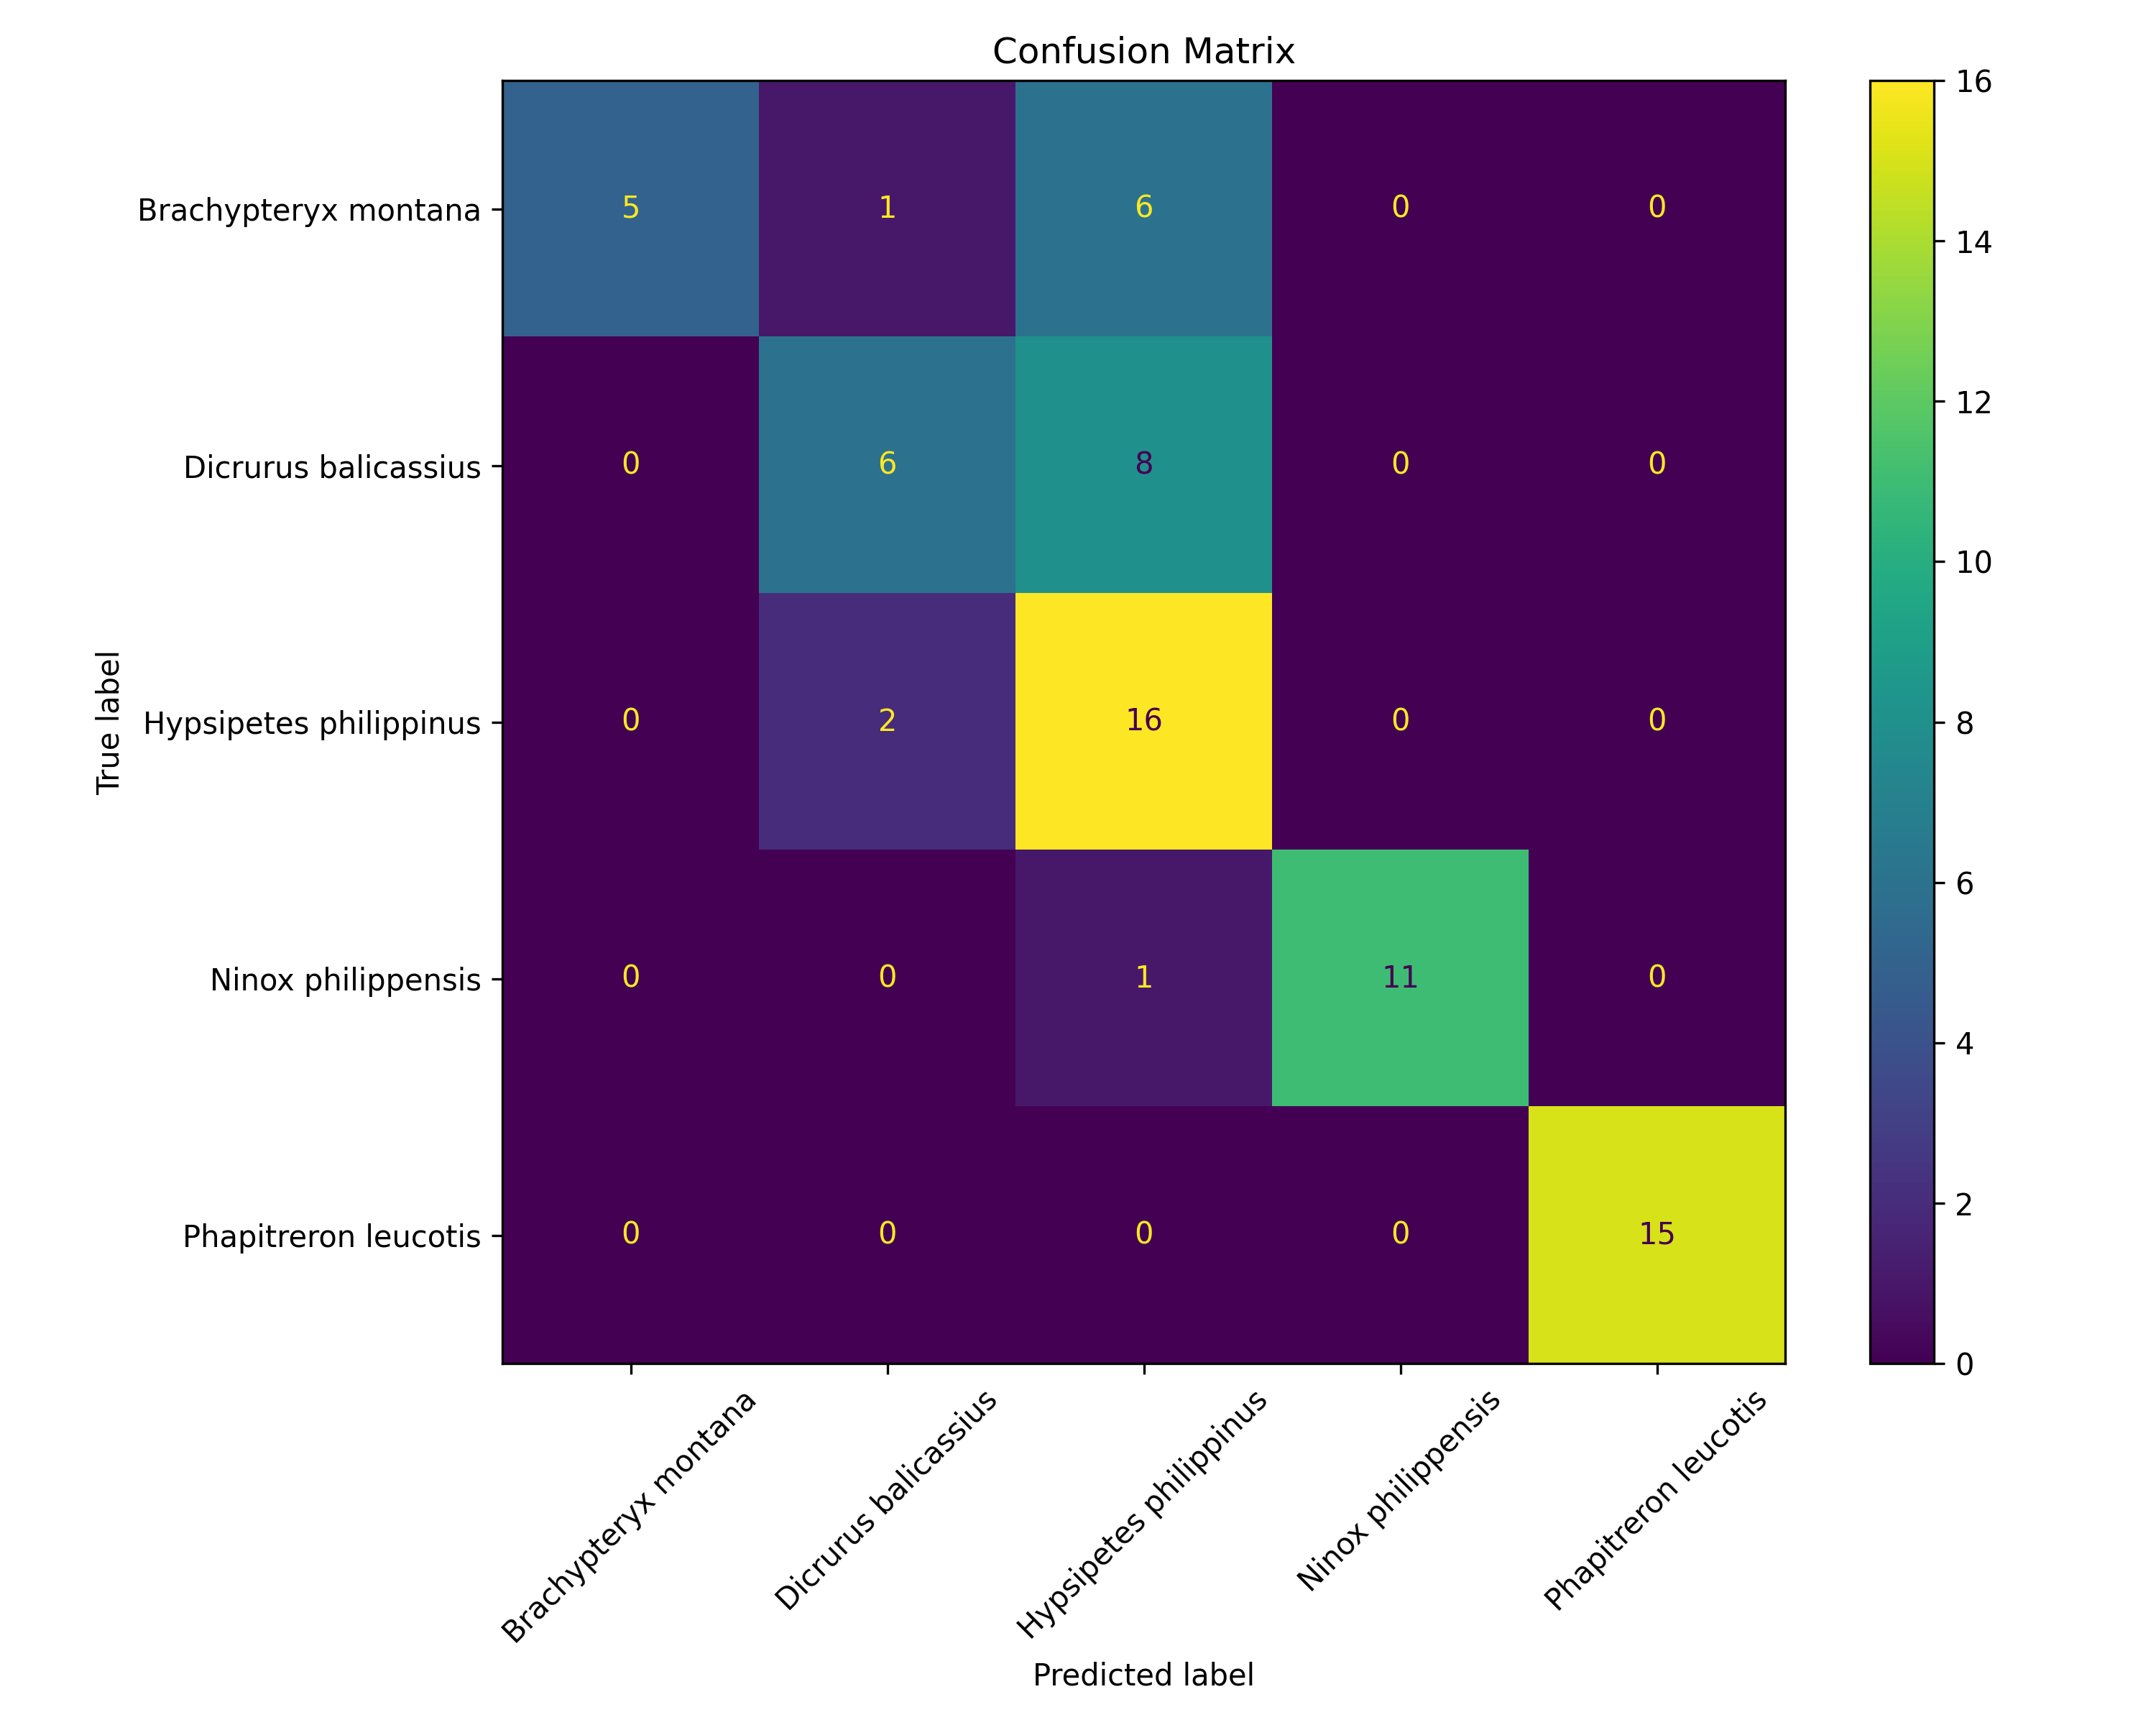
\includegraphics[width=0.80\textwidth]{figures/confusion_matrix.png}
\caption{Confusion matrix of the final model on the held-out test set.}
\label{fig:confusion-matrix}
\end{figure}

The confusion matrix in Figure~\ref{fig:confusion-matrix} confirms that the model was more reliable for some species than others. The observed errors may be attributed to overlapping acoustic characteristics, background noise, recording-condition differences, and the limited number of training samples. Overall, the final accuracy of approximately 75\% indicates that handcrafted acoustic features with classical machine learning provide a feasible baseline for selected Philippine bird species classification, but further improvement is needed for robust field deployment.

\section{Conclusion and Future Work}

This study developed and evaluated a classical machine learning pipeline for classifying selected Philippine bird species from audio recordings. Recordings were collected from Xeno-canto, processed into standardized audio clips, and represented using handcrafted acoustic features such as MFCCs, spectral descriptors, and temporal features. Several traditional classifiers were compared, including Logistic Regression, SVM, Random Forest, Extra Trees, Gradient Boosting, K-Nearest Neighbors, and XGBoost.

The results showed that tree-based ensemble models performed competitively during cross-validation. Random Forest achieved the highest mean accuracy among the baseline models, while Extra Trees achieved the highest mean macro F1-score. After hyperparameter tuning, XGBoost obtained the highest cross-validation macro F1-score of 0.7714. On the final held-out test set, the selected final model achieved an accuracy of 0.7465 and a macro F1-score of 0.74.

These findings suggest that classical machine learning with handcrafted acoustic features can serve as a useful baseline for Philippine bird species classification. However, the system was limited by the relatively small dataset size, background noise, variation in recording conditions, and the use of recording-level labels rather than manually segmented bird vocalizations.

Future work may improve the system by increasing the number of recordings, adding more bird species, applying more advanced noise reduction, and using syllable-level or segment-level classification. Deep learning models such as convolutional neural networks on mel spectrograms may also be explored and compared with the classical machine learning baseline developed in this study.

\bibliographystyle{splncs04}
\bibliography{references}

\end{document}